\documentclass[10pt,twocolumn]{article}
\usepackage[margin=0.75in]{geometry}
\usepackage{booktabs,graphicx,hyperref,amsmath}
\usepackage[T1]{fontenc}
\usepackage{lmodern}
\usepackage{xcolor}
\hypersetup{colorlinks=true,linkcolor=black,urlcolor=blue!50!black,citecolor=black}
\setlength{\tabcolsep}{4pt}

\title{Vision Can't Feel: Minimal Pairs for Contact-Dependent Robot Success Judgment}
\author{Anya Louni}
\date{October 2026}

\begin{document}
\maketitle

\begin{abstract}
Vision-language models (VLMs) are increasingly used to judge whether a robot finished its task. Recent work found these judges near chance when success depends on contact. We study that failure under control. We generate \emph{minimal pairs} in MuJoCo: two snapshots of the same randomized scene, one a success and one a failure that differs by a few millimeters (touching vs.\ hovering, grasped vs.\ beside, seated vs.\ on the rim, pressed vs.\ barely pressed, touching a wall vs.\ short of it). We compare free VLM judges with tiny classifiers on three deliberately degraded, low-cost sensor signals: a fingertip contact switch, gripper effort, and a single-axis wrist force. We also search for the largest physical failure that still fools each VLM. NUMBERS\_ABSTRACT
\end{abstract}

\section{Motivation}
A success detector gates retries, rewards, and data collection. A false success is the costly error: the robot moves on while the task silently failed. For contact-dependent tasks the evidence is often a millimeter gap or a force, which a camera at 640 pixels sees poorly or not at all. Cheap sensors measure contact directly. We ask how far that intuition holds when the sensors are realistically noisy, and where it breaks.

\section{Related work}
FailBench~\cite{failbench} evaluates 13 VLM detectors on 2{,}197 real and simulated attempts. Detection is near saturation when success shows as object motion and near chance on contact-rich assembly (no model above 0.60 balanced accuracy on its REASSEMBLE subset), with a bias toward predicting success. It uses vision only and names force-torque as future work. Guardian~\cite{guardian}, AHA~\cite{aha} and RoboFAC~\cite{robofac} train vision-language failure detectors from perturbed demonstrations; all are vision-only. Force and touch appear in policies (e.g.\ force-aware VLAs) rather than as success judges, and classical multimodal anomaly detectors predate VLM judges. To our knowledge no prior work compares cheap non-visual sensors with VLM judges on the same attempts. The vision-side finding is therefore not new; our contribution is the controlled minimal-pair setting, the degraded-sensor comparison, fusion, and the physical attacker. FailBench data was not yet released when we checked, so we could not report on its subset.

\section{Setup}
\paragraph{Simulation.} MuJoCo 3.17 with the Menagerie Franka Panda (gravity compensation, position actuators, damped least-squares IK, guarded moves that stop at 8\,N of tared wrist force). Five tasks, each with a matched failure: \textbf{stack} (held cube touching the base vs.\ hovering), \textbf{grasp} (closed on the cube vs.\ beside it), \textbf{button} (pressed past a 4\,mm click vs.\ less), \textbf{peg} (seated vs.\ on the rim), \textbf{push} (block against a wall vs.\ short of it).
\paragraph{Ground truth.} Explicit rules on simulator state after a 2\,s stability hold with controls frozen: contact force between the right bodies, cap displacement, peg depth plus floor contact, and for grasp a lift test. Images and sensors are captured \emph{before} the hold, at the moment a judge would decide. A pair counts only if its labels come out opposite.
\paragraph{Randomization.} Seeded per pair: key and fill light, table tint, object colors from a palette, three camera poses (one raised oblique, two low profile views), and 0 to 4 distractors kept out of camera sight lines.
\paragraph{Pairs.} Table~\ref{tab:pairs} shows failure magnitudes and the median front-view pixel difference within pairs.
\begin{table}[t]\centering\small\begin{tabular}{lrrr}
\toprule
Task & Pairs & Failure magnitude (mm) & Front pixel diff \\
\midrule
stack & 40 & 0.5--2.0 & 3.6 (median) \\
grasp & 40 & 1.1--3.9 & 24.8 (median) \\
button & 40 & 0.4--2.4 & 5.3 (median) \\
peg & 40 & 0.5--3.9 & 10.3 (median) \\
push & 40 & 0.6--3.0 & 3.7 (median) \\
\bottomrule
\end{tabular}\caption{Scaled set: minimal pairs per task.}\label{tab:pairs}\end{table}
\paragraph{Cheap sensors.} From the simulator at 100\,Hz: fingertip touch (thresholded at 0.3\,N into a binary switch per finger), gripper actuator force (a motor-current proxy), and wrist force along the tool axis only. Degradation per unit strength: switch flips 2\%, 30\,ms latency; effort noise 0.6\,N, 10-bit over $\pm$40\,N, drift up to 0.8\,N; force noise 0.5\,N, 8-bit over $\pm$30\,N, offset up to 1.5\,N, drift up to 1\,N; 2\% dropped samples; 20\,ms latency. Twelve summary features feed logistic regression and a small gradient-boosted tree, trained on 600 samples from seeds disjoint from every test set.
\paragraph{VLM judges.} Free tiers only: Gemini 3.5 Flash, Gemini 3.1 Flash-Lite and Gemma 4 31B through Google AI Studio; Qwen 3.8 27B through Groq; Qwen2.5-VL 3B and Moondream 1.8B through local Ollama on a CPU laptop (images downscaled to 384\,px for these two). Each gets a task description and one front image (single view) or all three views (multi-view), and returns JSON with a verdict and a confidence. Every answer is cached by (model, image hashes, prompt). Calibration uses the stated confidence.
\paragraph{Fusion.} Logistic regression on sensor features plus the VLM's P(success), 5-fold cross-validated on the test set with folds grouped by pair.

\section{Results}
\paragraph{Main comparison.} Table~\ref{tab:large} is the scaled set (400 samples). Table~\ref{tab:small} adds all models and multi-view on the 100-sample set. Free-tier daily quotas stopped some models early; the Coverage column says how many samples each judge answered, and metrics use only those.
\begin{table*}[t]\centering\small\begin{tabular}{lrrrrr}
\toprule
Judge & Coverage & Bal. acc. & False-succ. & False-fail. & ECE \\
\midrule
sensor\_gboost & all & 0.89 & 12\% & 10\% & 0.06 \\
sensor\_logreg & all & 0.89 & 11\% & 12\% & 0.04 \\
fusion: gemini/gemini-3.1-flash-lite (single) + sensors & 150/400 & 0.88 & 11\% & 13\% & 0.06 \\
gemini/gemini-3.1-flash-lite (single) & 150/400 & 0.55 & 53\% & 36\% & 0.45 \\
ollama/moondream:1.8b (single) & 8/400 & 0.50 & 100\% & 0\% & 0.17 \\
\bottomrule
\end{tabular}\caption{Scaled set (400 samples). Sorted by balanced accuracy.}\label{tab:large}\end{table*}
\begin{table*}[t]\centering\small\begin{tabular}{lrrrrr}
\toprule
Judge & Coverage & Bal. acc. & False-succ. & False-fail. & ECE \\
\midrule
fusion: gemini/gemma-4-31b-it (single) + sensors & 83/100 & 0.87 & 8\% & 19\% & 0.10 \\
sensor\_logreg & all & 0.86 & 14\% & 14\% & 0.06 \\
sensor\_gboost & all & 0.86 & 12\% & 16\% & 0.10 \\
fusion: ollama/moondream:1.8b (single) + sensors & 100/100 & 0.86 & 8\% & 20\% & 0.10 \\
fusion: gemini/gemini-3.1-flash-lite (multi) + sensors & 57/100 & 0.86 & 10\% & 18\% & 0.12 \\
fusion: gemini/gemini-3.1-flash-lite (single) + sensors & 100/100 & 0.85 & 8\% & 22\% & 0.13 \\
fusion: ollama/qwen2.5vl:3b (single) + sensors & 100/100 & 0.85 & 10\% & 20\% & 0.10 \\
fusion: groq/qwen/qwen3.8-27b (single) + sensors & 93/100 & 0.84 & 11\% & 22\% & 0.11 \\
fusion: gemini/gemini-3.5-flash (single) + sensors & 41/100 & 0.78 & 24\% & 20\% & 0.18 \\
gemini/gemini-3.1-flash-lite (multi) & 57/100 & 0.65 & 45\% & 25\% & 0.35 \\
gemini/gemini-3.5-flash (single) & 41/100 & 0.61 & 52\% & 25\% & 0.34 \\
gemini/gemini-3.1-flash-lite (single) & 100/100 & 0.60 & 46\% & 34\% & 0.40 \\
groq/qwen/qwen3.8-27b (single) & 93/100 & 0.57 & 43\% & 43\% & 0.36 \\
gemini/gemma-4-31b-it (single) & 83/100 & 0.56 & 38\% & 51\% & 0.42 \\
gemini/gemma-4-31b-it (multi) & 9/100 & 0.55 & 40\% & 50\% & 0.43 \\
ollama/moondream:1.8b (single) & 100/100 & 0.50 & 100\% & 0\% & 0.23 \\
ollama/qwen2.5vl:3b (single) & 100/100 & 0.50 & 100\% & 0\% & 0.44 \\
\bottomrule
\end{tabular}\caption{Small set (100 samples), all judges including multi-view. Partial coverage reflects free-tier quotas.}\label{tab:small}\end{table*}
\begin{table}[t]\centering\small\resizebox{\columnwidth}{!}{\begin{tabular}{lrrrrr}
\toprule
Judge & stack & grasp & button & peg & push \\
\midrule
sensor\_gboost & 1.00 & 1.00 & 0.97 & 1.00 & 0.46 \\
sensor\_logreg & 0.94 & 1.00 & 1.00 & 0.99 & 0.50 \\
fusion: gemini/gemini-3.1-flash-lite (single) + sensors & 0.97 & 1.00 & 0.93 & 1.00 & 0.50 \\
gemini/gemini-3.1-flash-lite (single) & 0.50 & 0.67 & 0.57 & 0.60 & 0.43 \\
ollama/moondream:1.8b (single) & -- & 0.50 & 0.50 & 0.50 & 0.50 \\
\bottomrule
\end{tabular}}\caption{Balanced accuracy by task, scaled set.}\label{tab:task}\end{table}
RESULTS\_TEXT

\paragraph{Where sensors fail.} The single-axis wrist force runs along the tool, so a sideways push barely registers, and the fingertip switch only sees the push if the contact lands inside its zone. Table~\ref{tab:task} shows the push column. Sensor classifiers also do not transfer across tasks (Table~\ref{tab:loto}): a model trained on four tasks is near chance on the fifth, because the same signal means different things in different tasks.
\begin{table}[t]\centering\small\begin{tabular}{lrr}
\toprule
Held-out task & Bal. acc. & False-succ. \\
\midrule
stack & 0.50 & 100\% \\
grasp & 1.00 & 0\% \\
button & 0.66 & 68\% \\
peg & 0.50 & 100\% \\
push & 0.50 & 0\% \\
\bottomrule
\end{tabular}\caption{Sensor classifier trained on four tasks, tested on the held-out one.}\label{tab:loto}\end{table}

\paragraph{Noise robustness.} Table~\ref{tab:sweep} and Figure~\ref{fig:sweep} scale every degradation together. SWEEP\_TEXT
\begin{table}[t]\centering\small\begin{tabular}{lrr}
\toprule
Noise strength & Bal. acc. & False-succ. \\
\midrule
0 & 0.97 & 2\% \\
0.5 & 0.90 & 10\% \\
1 & 0.89 & 11\% \\
2 & 0.82 & 18\% \\
4 & 0.74 & 20\% \\
8 & 0.66 & 32\% \\
16 & 0.60 & 41\% \\
32 & 0.49 & 54\% \\
\bottomrule
\end{tabular}\caption{Sensor classifier vs.\ noise strength (1 = default cheap hardware).}\label{tab:sweep}\end{table}
\begin{figure}[t]\centering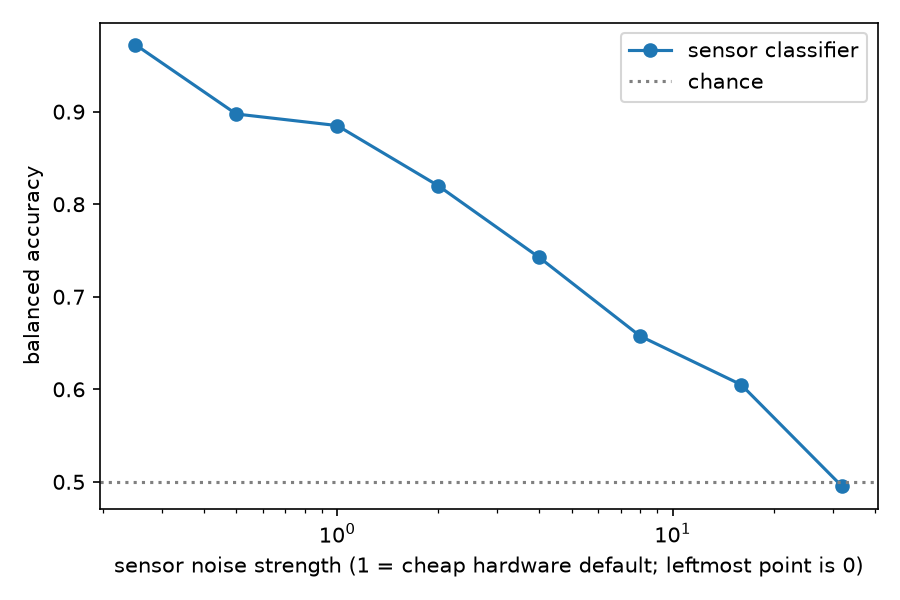
\includegraphics[width=\columnwidth]{../results/large/noise_sweep.png}\caption{Sensor classifier balanced accuracy vs.\ noise strength; dashed: best VLM on the same set.}\label{fig:sweep}\end{figure}

\paragraph{Calibration.} Figure~\ref{fig:rel} plots reliability. CALIB\_TEXT
\begin{figure}[t]\centering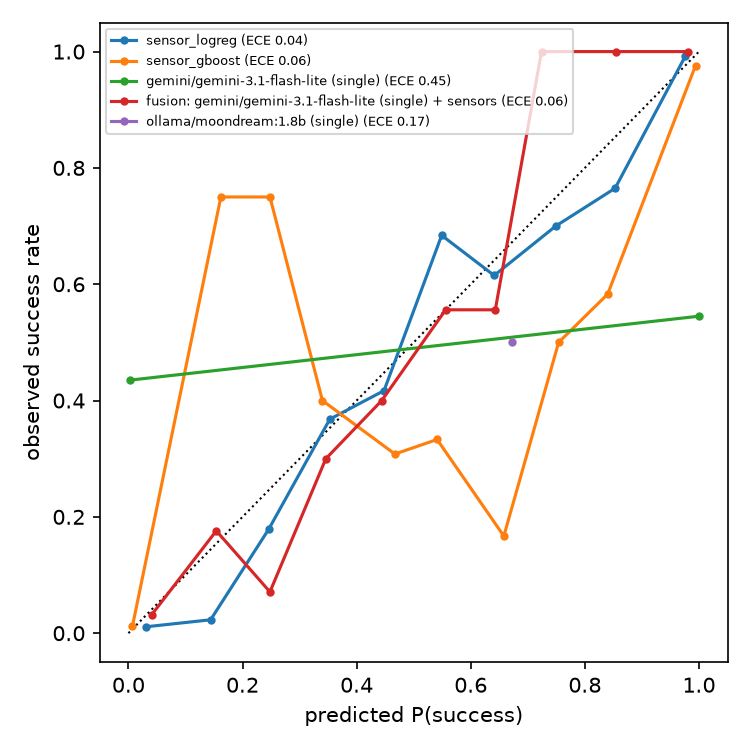
\includegraphics[width=\columnwidth]{../results/large/reliability.png}\caption{Reliability diagrams on the scaled set. VLM confidence is self-reported.}\label{fig:rel}\end{figure}

\paragraph{Millimeters to fool.} For each model, task and scene the attacker climbs a ladder of failure magnitudes (0.5 to 16\,mm; 0.25 to 3.7\,mm below the click for the button), bisects between the largest fooled and smallest not-fooled value, then runs four LLM-proposed mutations (magnitude, light, camera height) that see all previous results. Every candidate is re-simulated and discarded if ground truth turns into success. Table~\ref{tab:attack} reports the largest failure still judged a success, averaged over two scenes; Table~\ref{tab:transfer} re-judges every fooling scene with the other model and the sensor classifier. ATTACK\_TEXT
\begin{table}[t]\centering\small\resizebox{\columnwidth}{!}{\begin{tabular}{lrrrrr}
\toprule
Model & stack & grasp & button & peg & push \\
\midrule
gemini/gemini-3.1-flash-lite & 11.2 & 0.0 & -- & -- & -- \\
ollama/moondream:1.8b & 16.0 & 16.0 & 3.7 & 16.0 & 16.0 \\
\bottomrule
\end{tabular}}\caption{Millimeters to fool (largest failure judged success; mean of 2 scenes).}\label{tab:attack}\end{table}
\begin{table}[t]\centering\small\IfFileExists{tables/transfer.tex}{\begin{tabular}{lr}
\toprule
Judge & Also says success \\
\midrule
gemini/gemini-3.1-flash-lite & 9/41 \\
ollama/moondream:1.8b & 15/15 \\
sensor classifier & 6/115 \\
\bottomrule
\end{tabular}}{Transfer run pending.}\caption{Fooling scenes re-judged by other judges.}\label{tab:transfer}\end{table}

\section{Limitations}
Simulation only; nothing here is validated on hardware, and simulated touch and force are cleaner than real ones even after degradation. The failures are synthetic and drawn from five tasks we designed, so the sensor features fit those tasks; leave-one-task-out results show they do not generalize. The minimal pairs are hard by construction, so VLM accuracy here says little about natural failure distributions. Free-tier quotas limited coverage for several models, and local models ran on downscaled images. VLM confidence is self-reported text, not a probability. We used one prompt per task and did not tune prompts per model. Two scenes per task in the attacker is small. Fusion is cross-validated on the test set rather than trained on separate VLM-labelled data.

\section{Reproducibility}
Code (MIT), the dataset with images, sensor traces, simulator states, ground truth and every model answer (CC BY 4.0), and a one-command script are public. Cached answers make reruns free.

\begin{thebibliography}{9}\small
\bibitem{failbench} Z.~Navasardyan, T.~Danielyan, H.~Davtyan. FailBench: How Reliable are VLMs at Judging Robot Task Success? arXiv:2609.03611, 2026.
\bibitem{guardian} P.~Pacaud, R.~Garcia, S.~Chen, C.~Schmid. Guardian: Detecting Robotic Planning and Execution Errors with Vision-Language Models. arXiv:2512.01946, 2025.
\bibitem{aha} AHA: A Vision-Language-Model for Detecting and Reasoning Over Failures in Robotic Manipulation. ICLR 2025, arXiv:2410.00371.
\bibitem{robofac} W.~Lu et al. RoboFAC: A Comprehensive Framework for Robotic Failure Analysis and Correction. arXiv:2505.12224, 2025.
\end{thebibliography}
\end{document}
